\tikzstyle{input_neuron}=[circle,draw=red!50,fill=red!10,thick,minimum size=6mm]
\tikzstyle{hidden_neuron}=[circle,draw=blue!50,fill=cyan!10,thick,minimum size=6mm]
\tikzstyle{output_neuron}=[circle,draw=green!50,fill=green!10,thick,minimum size=6mm]
\tikzstyle{input}=[circle,draw=black!50,fill=black!20,thick,minimum size=6mm]

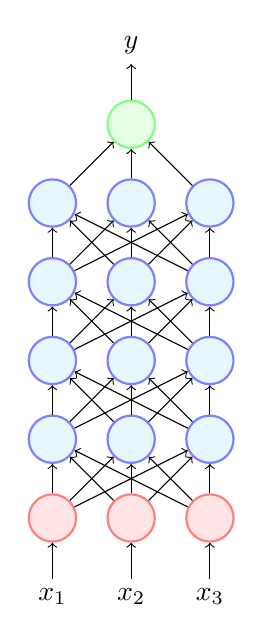
\begin{tikzpicture}
					
	\node [input_neuron] (neuron01) at (7,4.5){} ;
	\node [input_neuron] (neuron02) at (8,4.5){};
	\node [input_neuron] (neuron03) at (9,4.5){} ;
	\node (input0) at (7,3.5) {$x_{1}$};
	\node (input1) at (8,3.5) {$x_{2}$};
	\node (input2) at (9,3.5){$x_{3}$};
	
	\node [hidden_neuron] (neuron51) at (7,5.5){}  ;
	\node [hidden_neuron] (neuron52) at (8,5.5){}  ;
	\node [hidden_neuron] (neuron53) at (9,5.5){}  ;
	
	\node [hidden_neuron] (neuron11) at (7,6.5){}  ;
	\node [hidden_neuron] (neuron12) at (8,6.5){}  ;
	\node [hidden_neuron] (neuron13) at (9,6.5){}  ;
	\node [hidden_neuron] (neuron21) at (7,7.5){}  ;
	\node [hidden_neuron] (neuron22) at (8,7.5){}  ;
	\node [hidden_neuron] (neuron23) at (9,7.5){}  ;
	\node [hidden_neuron] (neuron31) at (7,8.5){}  ;
	\node [hidden_neuron] (neuron32) at (8,8.5){}  ;
	\node [hidden_neuron] (neuron33) at (9,8.5){}  ;
	%\node [output_neuron] (neuron41) at (7,9.5)  ;
	\node [output_neuron] (neuron42) at (8,9.5){}  ;
	%\node [output_neuron] (neuron43) at (9,9.5)  ;
	
	%\node (output0) at (7,10.5){$y_1$};
	\node (output1) at (8,10.5){$y$};
	%\node (output2) at (9,10.5){$y_3$};
	
	\draw[->](neuron01) -- (neuron51);
	\draw[->](neuron01) -- (neuron52);
	\draw[->](neuron01) -- (neuron53);
	\draw[->](neuron02) -- (neuron51);
	\draw[->](neuron02) -- (neuron52);
	\draw[->](neuron02) -- (neuron53);
	\draw[->](neuron03) -- (neuron51);
	\draw[->](neuron03) -- (neuron52);
	\draw[->](neuron03) -- (neuron53);
	
	\draw[->](neuron51) -- (neuron11);
	\draw[->](neuron51) -- (neuron12);
	\draw[->](neuron51) -- (neuron13);
	\draw[->](neuron52) -- (neuron11);
	\draw[->](neuron52) -- (neuron12);
	\draw[->](neuron52) -- (neuron13);
	\draw[->](neuron53) -- (neuron11);
	\draw[->](neuron53) -- (neuron12);
	\draw[->](neuron53) -- (neuron13);
	
	\draw [->] (neuron11) -- (neuron21);
	\draw [->] (neuron11) -- (neuron22);
	\draw [->] (neuron11) -- (neuron23);
	\draw [->] (neuron12) -- (neuron21);
	\draw [->] (neuron12) -- (neuron22);
	\draw [->] (neuron12) -- (neuron23);
	\draw [->] (neuron13) -- (neuron21);
	\draw [->] (neuron13) -- (neuron22);
	\draw [->] (neuron13) -- (neuron23);
	
	\draw [->] (neuron21) -- (neuron31);
	\draw [->] (neuron21) -- (neuron32);
	\draw [->] (neuron21) -- (neuron33);
	\draw [->] (neuron22) -- (neuron31);
	\draw [->] (neuron22) -- (neuron32);
	\draw [->] (neuron22) -- (neuron33);
	\draw [->] (neuron23) -- (neuron31);
	\draw [->] (neuron23) -- (neuron32);
	\draw [->] (neuron23) -- (neuron33);
	
	%\draw [->] (neuron31) -- (neuron41);
	\draw [->] (neuron31) -- (neuron42);
	%\draw [->] (neuron31) -- (neuron43);
	%\draw [->] (neuron32) -- (neuron41);
	\draw [->] (neuron32) -- (neuron42);
	%\draw [->] (neuron32) -- (neuron43);
	%\draw [->] (neuron33) -- (neuron41);
	\draw [->] (neuron33) -- (neuron42);
	%\draw [->] (neuron33) -- (neuron43);
	
	%\draw[->] (neuron41) -- (output0);
	\draw[->] (neuron42) -- (output1);
	%\draw[->] (neuron43) -- (output2);
	
	\draw[->] (input0) -- (neuron01);
	\draw[->] (input1) -- (neuron02);
	\draw[->] (input2) -- (neuron03);
	
\end{tikzpicture}